
% Chapter Template

\chapter{Structure Depth Dataset}

\label{Chapter4:Dataset} 

%----------------------------------------------------------------------------------------
%----------------------------------------------------------------------------------------
%\url{https://fenix.tecnico.ulisboa.pt/downloadFile/1689244997256744/Thesis.pdf}

In this Chapter, We present our dataset created using Structure Sensor and we call it as \textbf{Structure Depth} dataset. The entire chapter is divided in to three sections. In the first section we discuss the technical details of the Structure Sensor and followed by the methods involved in creating this dataset. The last part of this chapter is about the various pre processing methods we used to performed for specific experimental setups.


\section{Structure Depth Dataset Overview} 

Our aim in this work is to deliver a robust system for depth prediction as seen in the Figure \ref{fig:Proposed_Model} for a portable hand held mobile device. In our case it is an Ipad integrated with Structure sensor. In order minimize the difference between the predicted depth maps and depth map generated from Structure sensor we need to train with the similar dataset. We have also validated this in our experiments which will be discussed below in Section \ref{Chapter6:Results}. As discussed in the section \ref{Chapeter1:Topic_Description}, this will also help us to study the effect of different camera and sensor properties on diffrent environment.\\

As we have seen earlier in Chapter \ref{Chapter3:RelatedWork}, there are multiple datasets available but almost none fit our context. As we are already exploiting the depth features from NYU V2 for general prediction, we would like to produce a dataset which is solely application based. Here our application is mobile device, particularly IOS, we generate the dataset using an Ipad. This will not only make the intrinsic parameters to be learned by the network but also particularize for IOS based devices. As we use Ipad as integration, all the RGB Images are received from the Ipad's camera. The features we want the neural network to learn and predict should have the same camera intrinsic parameters in order to decrease the amount of pre processing of the dataset. Hence, We first calibrate Ipad with Structure Sensor before collecting the Dataset. Another major advantage of using Structure Sensor with an Ipad over Kinect is the resolution of RGB and Depth Images. While Kinect V2 has $512\times424$ Infrared camera resolution, Structure Sensor can go upto $640\times480$. \\

Our Dataset consist of 18 scenes and a total of 2675 images captured using an Apple iPad Pro version 12.9 (2015) model and a Structure Sensor by Occipital. The dataset majorly includes images from office and classrooms environments. It consist of RGB Images of $640\times480$ as 3 channel $\times$ 8 bit int and Raw Depth Images of 640 $\times$ 480 as 1 channel. Both of the images are saved using lossless compression. Later, we also perform some processing to synchronize RGB and depth images and to fill the holes of depth image which will be discussed later in this chapter. We also provide the camera extrinsic parameters as a numpy matrix of $4\times4$ which is useful for reconstruction of a scenario.\\


\subsection{Technical Specification of Structure Sensor}
The Structure Sensor \footnote{\url{https://structure.io/}} is a 3D scanner introduced by Occipital in 2014. As the name suggests, it uses Structured-Light-System(SLS) 3D scanning\cite{Kalantari}. It can be easily attached to an Ipad and with Structure SDK it enables us to generate good quality RGB image stream from Ipad and its realtive depth stream from Structure Sensor at the simultaneously. As it only weighs 95 grams and can be used as an extension to mobile device, it makes the sensor very portable. With possibility of recording 60 frames per second at a resolution of $640\times480$\cite{Kalantari}. When compared to Kinect V2, it has more depth image resolution. The comparison can be seen in table \ref{table:KinectVsStructureSensor}. The minimum range it can capture is 40 cm while it can capture till 4 m with fine precision. After 4 m the precision is not satisfactory enough to use it for the dataset. Occipital claims it has low frame-to-frame noise and provides 100\% fill rate on most of the materials. On the other hand Ipad Pro 12.9 provides us with an RGB video stream of $1920\times1080$ at 30 frames per second and $1080\times720$ at 60 frames per second. Ipad Pro also provides us with Camera extrinsic parameters which are useful for the reconstruction of the scenario.\\

\begin{table}[h]
\begin{tabular}{@{}lll@{}}
\toprule
\textbf{Features}                    & \textbf{Kinect V2}           & \textbf{Structure Sensor}         \\ \midrule
Depth Sensor Type           & ToF & SLS                 \\
RGB Camera Resolution       & $1920\times1080$, 30 fps & $1920\times1080$, 60 fps     \\
IR Camera Resolution        & $512\times424$, 30 fps   & $640\times480$, 60 fps                 \\ 
Field of View of IR Camera  & $70^\circ\times60^\circ$           & $58^\circ\times45^\circ$                         \\
Recommended Operative Range & 0.4 m - 3.5 m       & 0.4 m - 3.5 m                                  \\
           &                     & 
\end{tabular}
\caption{Comparison of Kinect V2 and Structure Sensor}
\label{table:KinectVsStructureSensor}
\end{table}

While these sensors are great devices they have some limitations. The distance they can measure is limited and they suffer from reflection problems on transparent, shiny or very matte and absorbing objects. Another limitation is holes generated by parallax effect happening due to difference in position of the camera of Ipad and Structure Sensor\cite{Kalantari}. In simpler terms, it works like human eyes. If we close one eye and then other, we notice a disparity. When there is an object we try to focus on, we see it through different angles. If the object is close enough, then sometimes one eye can see what is behind and other can not. This can be seen in figure \ref{fig:holes}. As a result, it produces a shadow of holes which can be seen in figure \ref{fig:holes2}.

\begin{figure}[h]
    \centering
    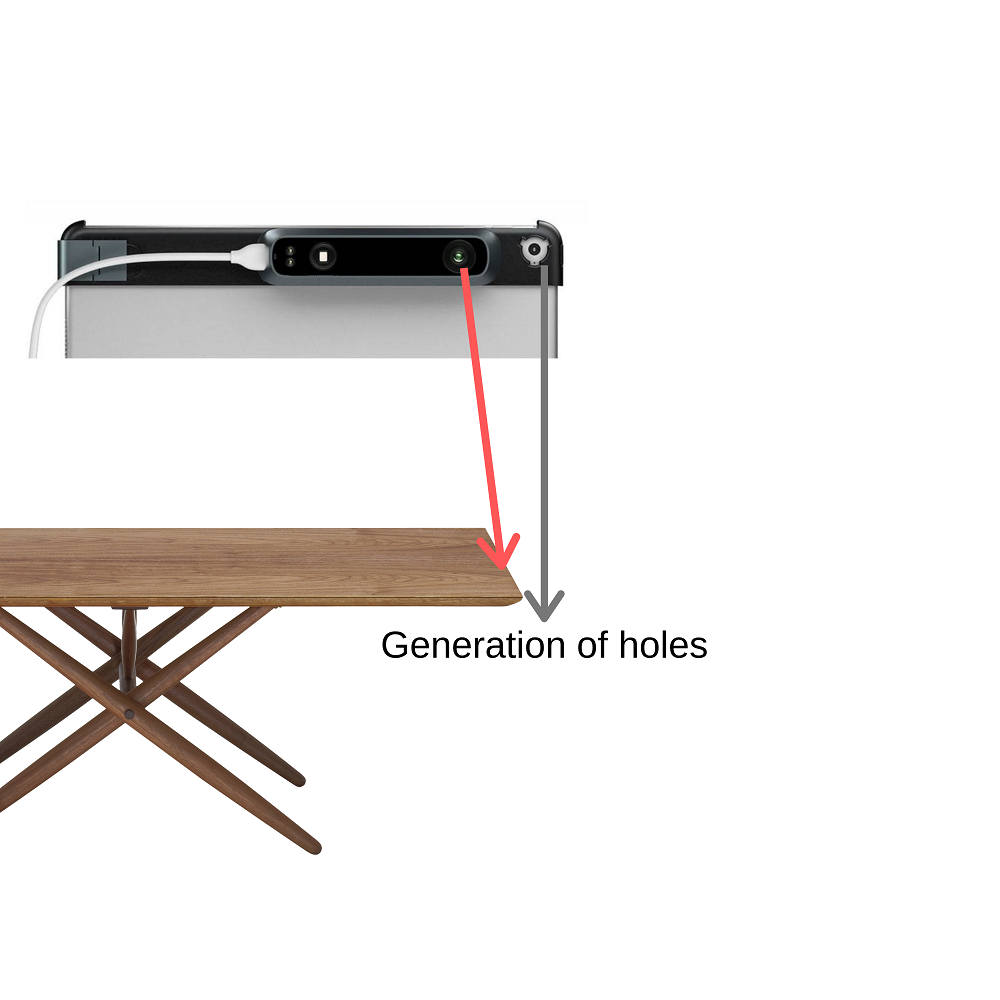
\includegraphics[scale=0.4]{Figures/holes.png}
    \caption{Generation of holes due to parallax}
    \label{fig:holes}
\end{figure}

\begin{figure}[h]
    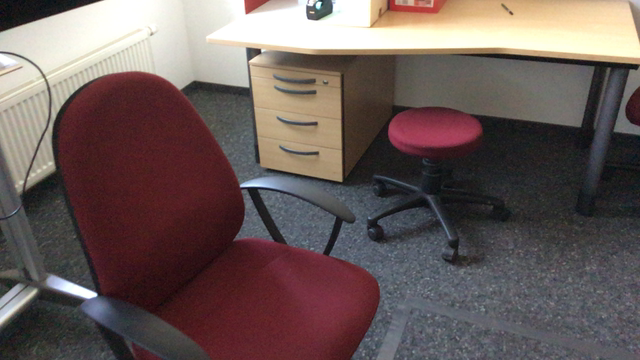
\includegraphics[scale=0.29]{Figures/RGB.png} 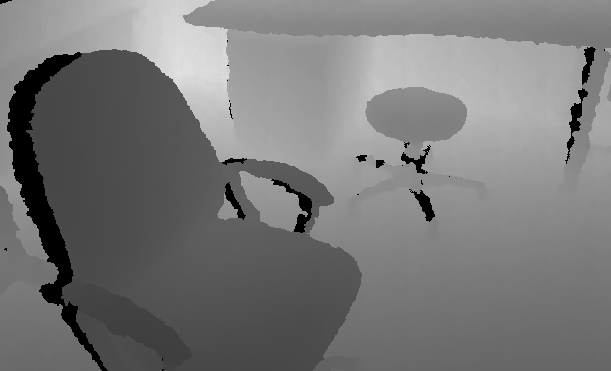
\includegraphics[scale=0.37]{Figures/Depth.png}
    \caption{Holes produced in depth image}
    \label{fig:holes2}
\end{figure}


\subsection{Dataset Collection}

A significant role in Machine Learning is played by Dataset and the collection of it makes most influence on the features that network learns. As the distance is limited in Structure Sensor and due to our scope of research we used indoor offices and classrooms to reduce the possibilities. While capturing the dataset, one should keep in mind that the network should learn only the novel features not the artifacts. One good instance of this would be recording the depth of a screen. Since, a screen has reflective black surface, it loses depth information resulting holes in depth image. \note{add img for screen} If we feed these images to the network, it might learn the features such as, screen is always at, let say x distance. Where x is pixel value we assign to such holes. This is not a good feature to be learned by the network instead it is an artifact. So before feeding it to the network we do some pre processing on the dataset which we will discuss next.\\

The generation of holes are usually due to the reflective surface of an object or the distance and position of the object\cite{geomar41830}. As a reflective/glossy surface generates holes, it should not be synthesized because this leads to distortion of depth information.

For the shadows happening due to parallax effect, we use inpainting \cite{zamir2018taskonomy} in order to minimize out the errors. Since, the accuracy decreases as the depth increases \cite{deptherror}, we remove all the pixels which are away more than 4 metres. This can be resolved using further predictions and post processing. All the information is registered in metres and  all of these processes were included while processing the raw depth information.\\

\subsection{Processing the Dataset}

After we have the distance in metres, we process the data before directly training the network on these images. Since these images still contain holes and precision less pixels, we pre process the images. Usually, very far pixels have less precision and results in holes as well\cite{deptherror}. It is a good idea to conserve those holes in order to reconstruct the environment by later predicting the future frames. Firstly, after we have the Depth images in metres, we flag \nadacn{We save all the holes by its pixel position or index} all the pixels more than 4000 cm to use them in the image later again as discussed later in this section.

As discussed earlier, the Depth images contains holes from shiny/glossy objects\cite{shiny}. In office environments, these holes are mostly generated by Computer Displays. Since we do not want our network to learn that all the screens are close(0 pixel), we interpolate these holes. We do this by inpainting the whole image. This fixes the issues of shadows made due to parallax as well. \\

In our first model, we made all the pixels more than 4 metres as 4 m like a wall but that was not a great idea. Since, our model learns what we feed it, the model now had no proper depth perception after 4 m \nadacn{this statements means after processing the depth precision  will increase more than 4 meater which is wrong} \shivam{its better to read the next line before making the comment}.\nadacn{still the statement does not convey everything.. you use "now (present tense)had (past tense) ?? I cannot corerent because I dont know what you want to say... You say, since there sensors depth sensing limitation is limited to a definite range in this case xxm the possibilities of  depth values beyond a threshold may not be with good precision, So as an approach we map all the pixel depth to a certain xx threshold... " } So, We decide to keep all the pixels more than 4 m as holes because we can reconstruct them using a video or multiple frames later if needed. Now, We have the whole image without any holes, but we want holes in our image. So, the next step is to re generate holes for the pixels more than 4000 cm. All the pixels we flagged are now changed to zero in order to create holes. \\

Our Image is now ready to be fed to the network but there is still one problem. The size of the Color Image and Depth Image does not match since they have different aspect ratios due to different camera sources. So, In the end we crop the depth image centre focused in order to make them compatible with each other.\\

\newpage